%Sexto ejercicio.
\documentclass{standalone}
\usepackage[utf8x]{inputenc}
\usepackage[T1]{fontenc}
\usepackage{PTSansNarrow}
\usepackage[usenames,dvipsnames,x11names,table,svgnames]{xcolor}
\usepackage{tikz}
\usetikzlibrary{babel,calc}
\begin{document}

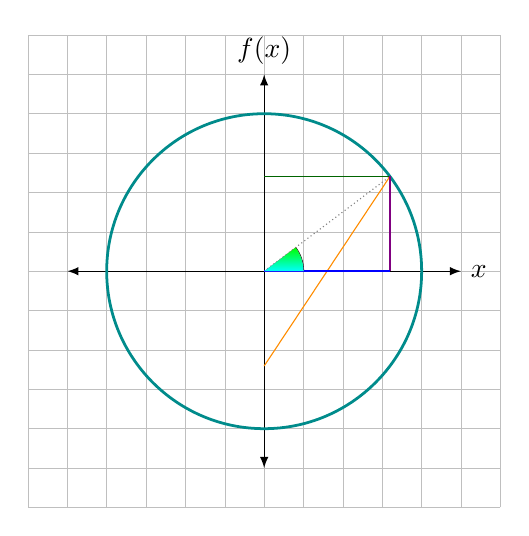
\begin{tikzpicture}
\def\t{37} %t\in[0,360]
\def\r{2}	%r>0.
\def\tangle{5mm}
\draw[gray!50, very thin, xstep = .5, ystep = .5] (-\r-1, -\r-1) grid (\r+1,\r+1);
%\clip (.15, 0);
%\clip (0, .5cm) circle ;
%\clip(.15, 0) circle (.5cm); %Investigar el uso de clip.
\draw (\tangle, 0) arc[start angle = 0, end angle = \t, radius =\tangle];
\draw[>=latex, <->] (-\r-0.5,0) -- (\r+0.5, 0) node[right] {$x$};
\draw[>=latex, <->] (0, -\r-0.5) -- (0, \r+0.5) node[above] {$f(x)$};
\draw[line width =1pt,DarkCyan](0,0) circle[radius = \r];
\draw[line width =.05pt, thin, densely dotted, gray] (0, 0) -- (\t:\r);
%dashed, thin, dotted,loosely
\draw[DarkGreen] (0,0) +(\t:\r) -- ++(0, {\r*sin(\t)});
\draw[DarkOrange] (0,0) +(\t:\r) -- ++(0, -{\r*sin(\t)});
\draw[line width =.7pt, red!50!blue](0,0) ++(\t:\r) -- ++(0, -{\r*sin(\t)});
\draw[line width =.7pt, blue] (0,0) -- (+{\r*cos(\t)}, 0);
\fill[magenta] (0,0) -- (\tangle, 0) arc[start angle = 0, end angle = \t, radius =\tangle] -- cycle;
\shade[top color = green, bottom color = cyan] (0,0) -- (\tangle, 0) arc[start angle = 0, end angle = \t, radius =\tangle] -- cycle;
\end{tikzpicture}

\end{document}